\documentclass[12pt,letterpaper,titlepage,en-US]{article}

\usepackage{basicstyle}
\usepackage{report}
%\usepackage{knit}

\usepackage{listings}
\usepackage{xcolor}


\definecolor{codegreen}{rgb}{0,0.6,0}
\definecolor{codegray}{rgb}{0.5,0.5,0.5}
\definecolor{codepurple}{rgb}{0.58,0,0.82}
\definecolor{backcolour}{rgb}{0.95,0.95,0.92}
 
\lstdefinestyle{mystyle}{
    backgroundcolor=\color{backcolour},   
    commentstyle=\color{codegreen},
    keywordstyle=\color{magenta},
    numberstyle=\tiny\color{codegray},
    stringstyle=\color{codepurple},
    basicstyle=\ttfamily\footnotesize,
    breakatwhitespace=false,         
    breaklines=true,                 
    captionpos=b,                    
    keepspaces=true,                 
    numbers=left,                    
    numbersep=5pt,                  
    showspaces=false,                
    showstringspaces=false,
    showtabs=false,                  
    tabsize=2
}
 
\lstset{style=mystyle}



\usepackage[toc,page]{appendix}

\newcommand{\hmwkTitle}{Project \#2}
\DTMsavetimestamp{DueDate}{2019-11-05T11:59:00+00:00}
\newcommand{\hmwkClass}{CS 6385.001}
\newcommand{\hmwkClassName}{Algorithmic Aspects of Telecommunication Networks}
\newcommand{\hmwkClassInstructor}{Instructor: Prof. Andras Farago}
\newcommand{\hmwkAuthorName}{Shyam Patharla}
\newcommand{\hmwkAuthorNetID}{sxp178231}




%
% Title Page
%

\title{
    \vspace{1in}
    \textmd{\textbf{\hmwkClassName \\\hmwkClass:\ \hmwkTitle }}\\
    \normalsize\vspace{0.1in}\small{Due\ on\ \DTMusedate{DueDate}\ at \DTMusetime{DueDate} }\\
    \vspace{0.1in}\large{\textit{\hmwkClassInstructor}}\\
    \vspace{0.5in}
\includegraphics[height=2.4em]{UTD_logo_BW}\\
    \vspace{2in}
}

\author{\textbf{\hmwkAuthorName\ \footnotesize{(\hmwkAuthorNetID)}} \\ }
\date{}
\makeindex

\begin{document}
\maketitle
\pagenumbering{Roman}

\tableofcontents

\pagebreak
\pagenumbering{arabic}

\section{Introduction}
\begin{itemize}
\item In this project, we try to implement the basic network design model
\item Give an input number of nodes, traffic demands between different nodes and a parameter k, our program outputs a network topology i.e a directed graph with links and capacities assigned to these links
\item We do this for range of values of k
\item  We also analyze how the cost and density of the output network vary with the value of k
\item We discuss the possible reasons for the above characteristics.
\end{itemize}

\section{Design Decisions}
\begin{itemize}
\item We implement the solution in the \textbf{Java} programming language
\item The program modules were run on a \textbf{Mac} operating system

\end{itemize}





\section{Solution Approach}

\subsection{Generating Input Examples}
\textit{Module 1} consists of generating input graphs for simulating the algorithm.
These parameters are then passed on to second module which runs the Nagamochi Ibaraki  algorithm on them. The graphs are generated as follows.

\begin{itemize}
\item For all examples, we set the number of nodes in the network to 20 i.e \textit{n} = 20.

\item The number of edges is taken from the set [19,190] in steps of 3 i.e. m=19,22,25,....190

\item For each pair of values of m and n we generate 5 graphs

\item  The m edges are selected randomly 
\item Self loops and parallel edges are avoided.



\end{itemize}




\subsection{Nagamochi Ibaraki Algorithm}
Module 2 receives input parameters from the first module (graph).

\begin{itemize}

\item All pairs shortest paths
\begin{itemize}
\item We compute the shortest distances between all pairs of nodes using the \textbf{FloydWarshall algorithm} i.e. and store them in a  matrix \textit{dist}

\item While computing the above \textit{dist} matrix, we also store the shortest paths between each pair of nodes (i,j) in the pred matrix. Each entry \textbf{pred\textsubscript{ij}} gives the node with \textbf{maximum} number in the shortest path between nodes i and j. 

\item \textbf{Special case:} If there is no node in the shortest path between i and j, pred\textsubscript{ij}=-1
\end{itemize}

\item Design Links and Capacities
\begin{itemize}
\item The \textit{capacities} matrix and \textit{links} matrix are initiated with all values equal to \textbf{zero}

\item Let S be the shortest path between nodes k and l, where k$\neq$l. For each edge (i,j) on S  
\begin{itemize}
\item If  \textbf{link\textsubscript{ij}} has not been set to 1, set it to 1 
\item The capacity of link\textsubscript{ij}  is incremented by \textbf{demand\textsubscript{kl}} 

\end{itemize}

\item The above process is repeated for each pair of nodes (k,l) where k$\neq$l.

\end{itemize}


\item The \textit{links} and \textit{capacities} matrices are passed on to Module 3, which analyzes how the total cost of the network and densities change with respect to our k parameter.


\subsection{Presentation of Results}
\begin{itemize}

\item Module 3 takes the output parameters of \textit{Module 2} i.e. the capacities and link matrices and computes
 \begin{itemize}
 \item the \textbf{total cost} of the network
 \item the \textbf{density} of the network i.e. the number of links with \textbf{non-zero} capacities divided by the maximum possible number of links which is N*(N-1)
 \end{itemize}
 
 \item The above computation is repeated for all k values
 
\item We then try to answer questions such as:
\begin{itemize}
\item How does the total cost of the network depend on k?
\item How does the density of the obtained network depend on k? 
\end{itemize}

\item We show some of the obtained network topologies graphically 
\end{itemize}

We present the execution of our project using the flow chart below.\\

  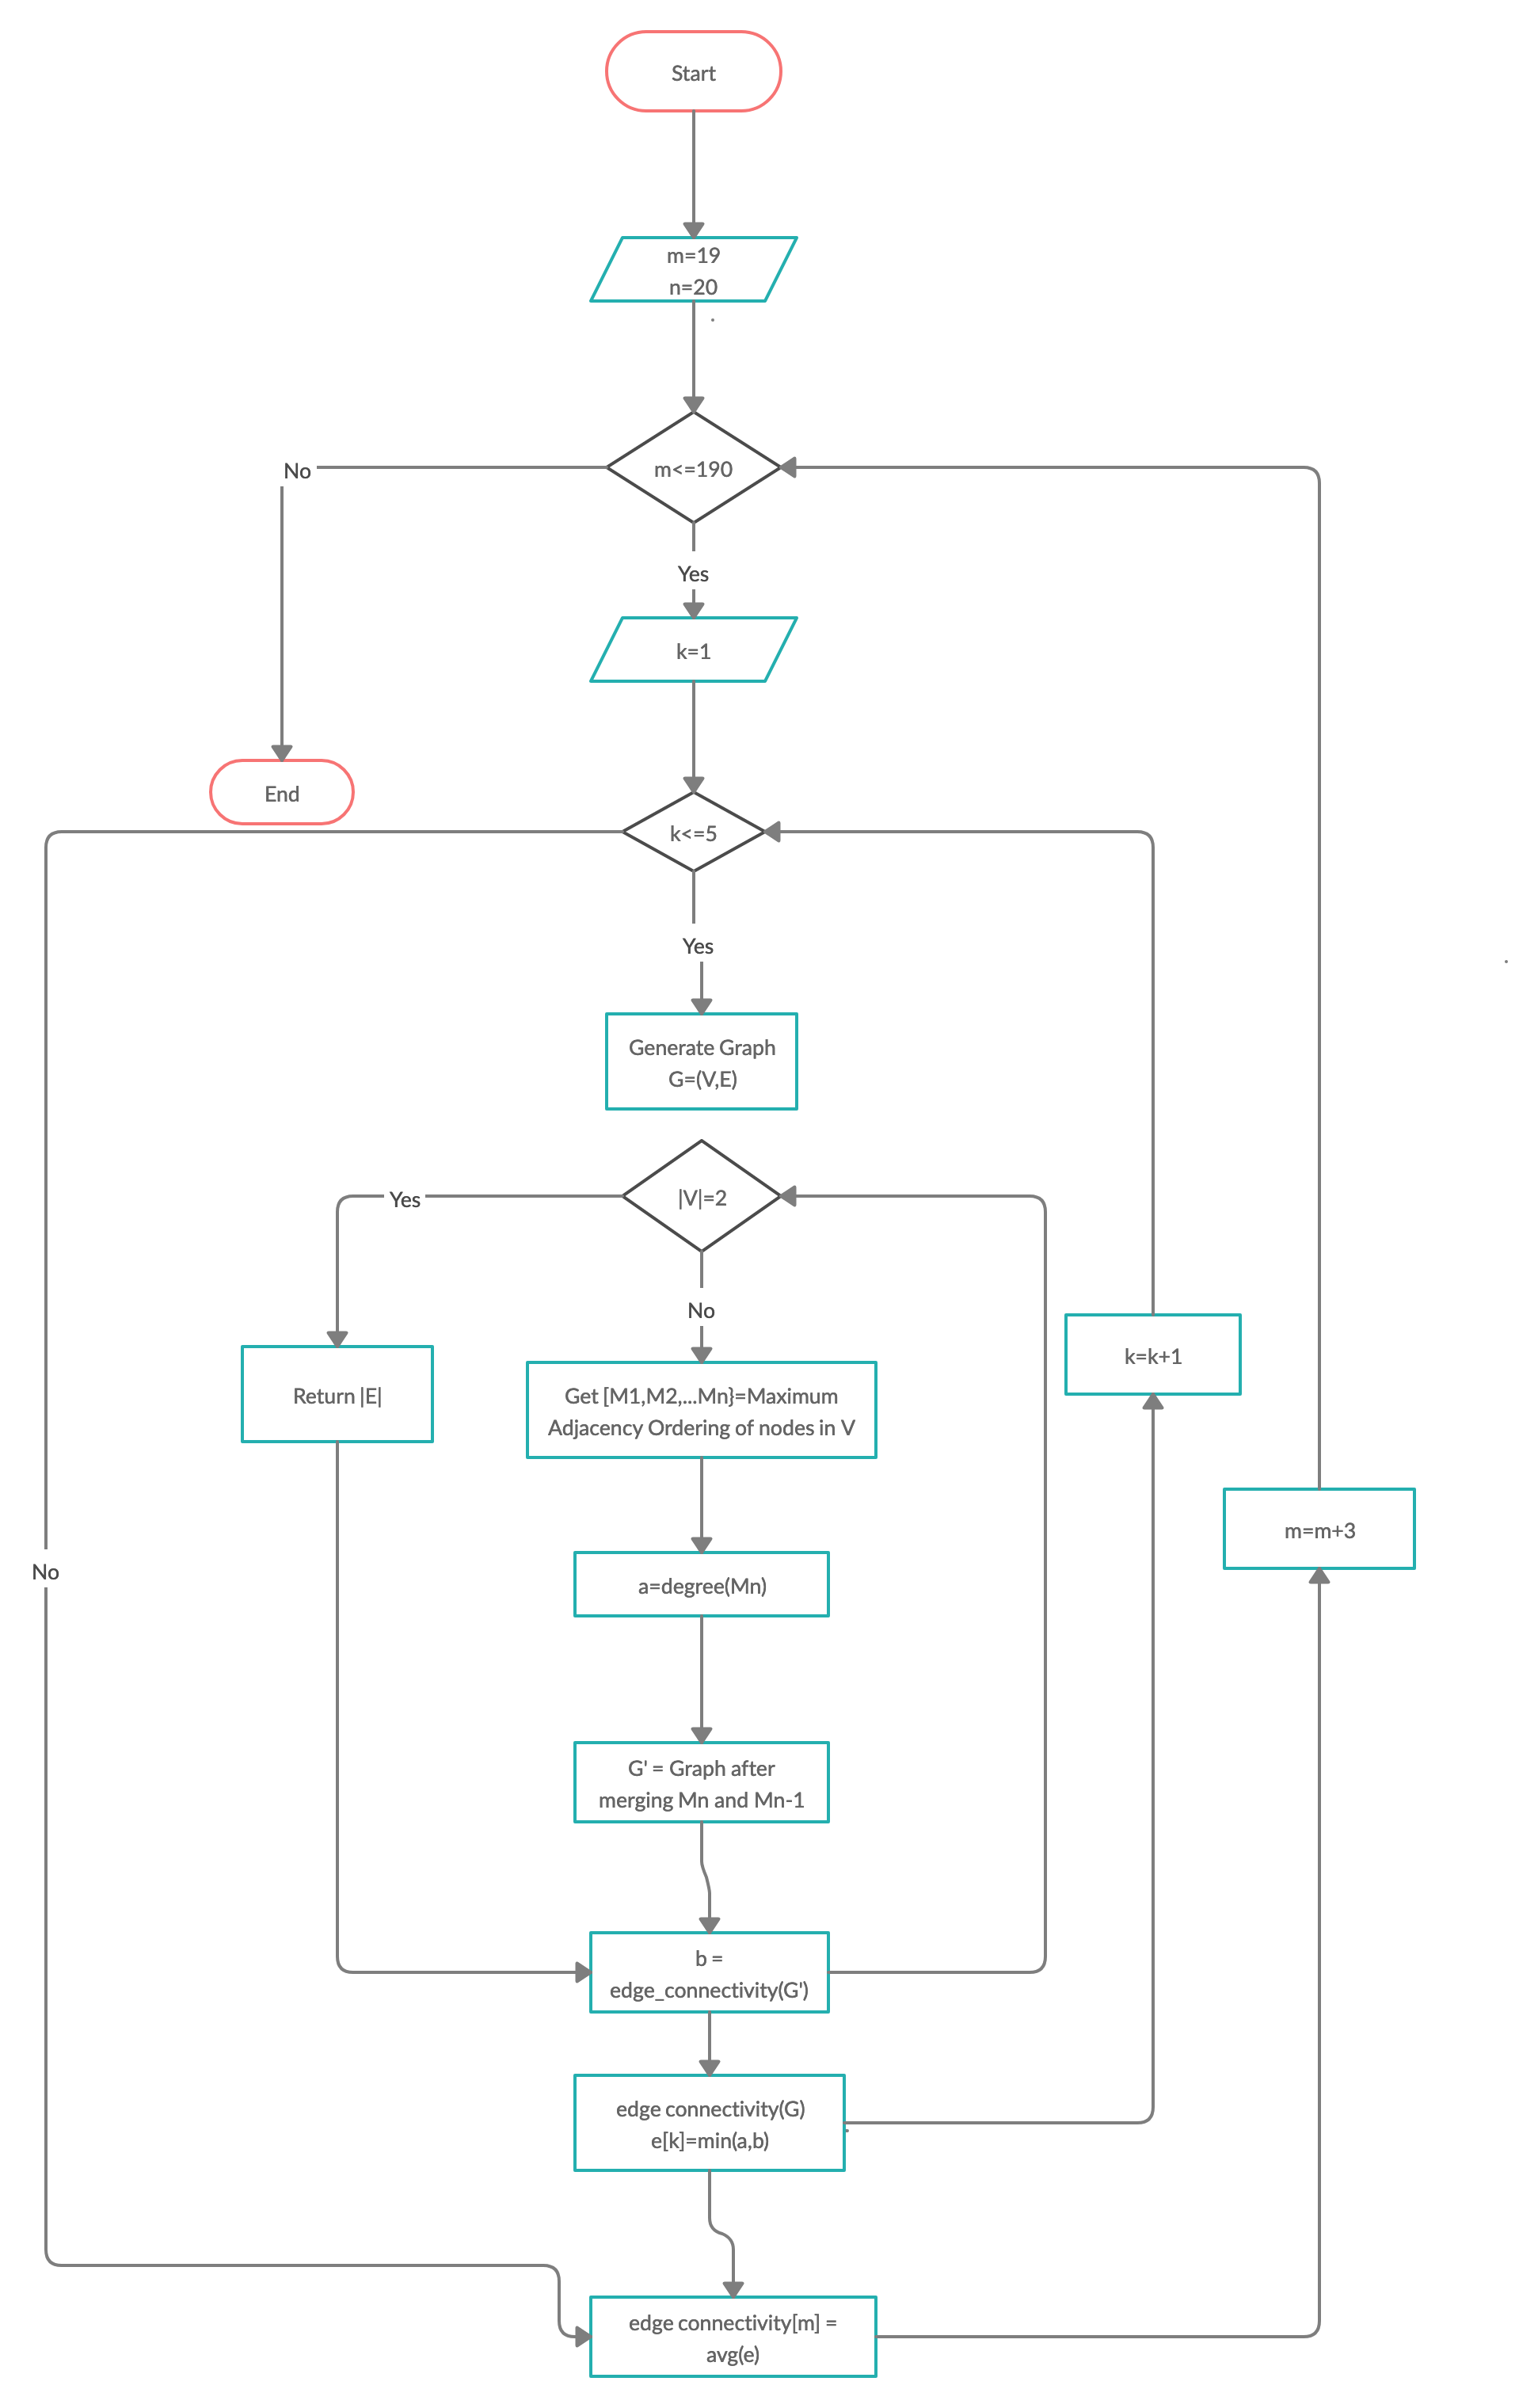
\includegraphics[scale=0.6]{fig/flowchart.png}
\end{itemize}


\section{Nagamochi Ibaraki Algorithm - Explanation}
\begin{itemize}
\item Suppose we have N vertices and the vertices are numbered from 1,2,...,N

\item For every pair of vertices i and j we define a path $\pi(i,j,r)$ which is  the shortest path from i to j that passes through vertices numbered atmost r.

\item This problem has a simple recursive structure

\item \textbf{Base Case}: The path $\pi(i,j,0)$ cannot pass through any vertices, so it is the edge(if any) between i an j

\item \textbf{Recursive Case}: The path $\pi(i,j,r)$ will have two cases
\begin{itemize}
\item The path does not pass through the vertex labeled r, so it must pass through the vertices numbered atmost r-1 $\implies \pi(i,j,r) = \pi(i,j,r-1)$

\item The path passes through the vertex labeled r. It will consist of the path from i to r and the path from r to j, each of which passes through vertices numbered atmost r-1 



\end{itemize}


\item We first try our hands at a straightforward dynamic programming approach, which is shown below





\item  We can simplify the algorithm by removing the third dimension. We can also modify the algorithm to support numbering the vertices arbitrarily
\begin{algorithm}[H]
    \caption{NagamochiIbarakiAlgorithm}
    \begin{algorithmic}[1]
        \Procedure{NagamochIbaraki}{$V,E$}
      
      \State n=nodes.length
      \If{$n=2$}
      \State return degree (y)
      \EndIf
      
        
        \State v[] = maximumAdjacencyOrdering(V)
        
        \State $x=v_{n-1}$
        \State $y=v_{n}$
        \State a=$degree(y)$
        \State$ G_{xy}$=graph created by merging nodes x and y
        \State b = NagamochiIbaraki$(V_{xy}, E_{xy})$
        \State return min(a,b)
        
     
     
      
        \EndProcedure
    \end{algorithmic}
    \end{algorithm}


\item The \textbf{dist} matrix gives the shortest path distances between all pairs of nodes.
\item 
The \textbf{pred} matrix gives the node with maximum number in the shortest path between any two nodes.
\end{itemize}

\section{Observations and Analysis}
\begin{itemize}


\item The program produces an output as shown in the figure below.\\

 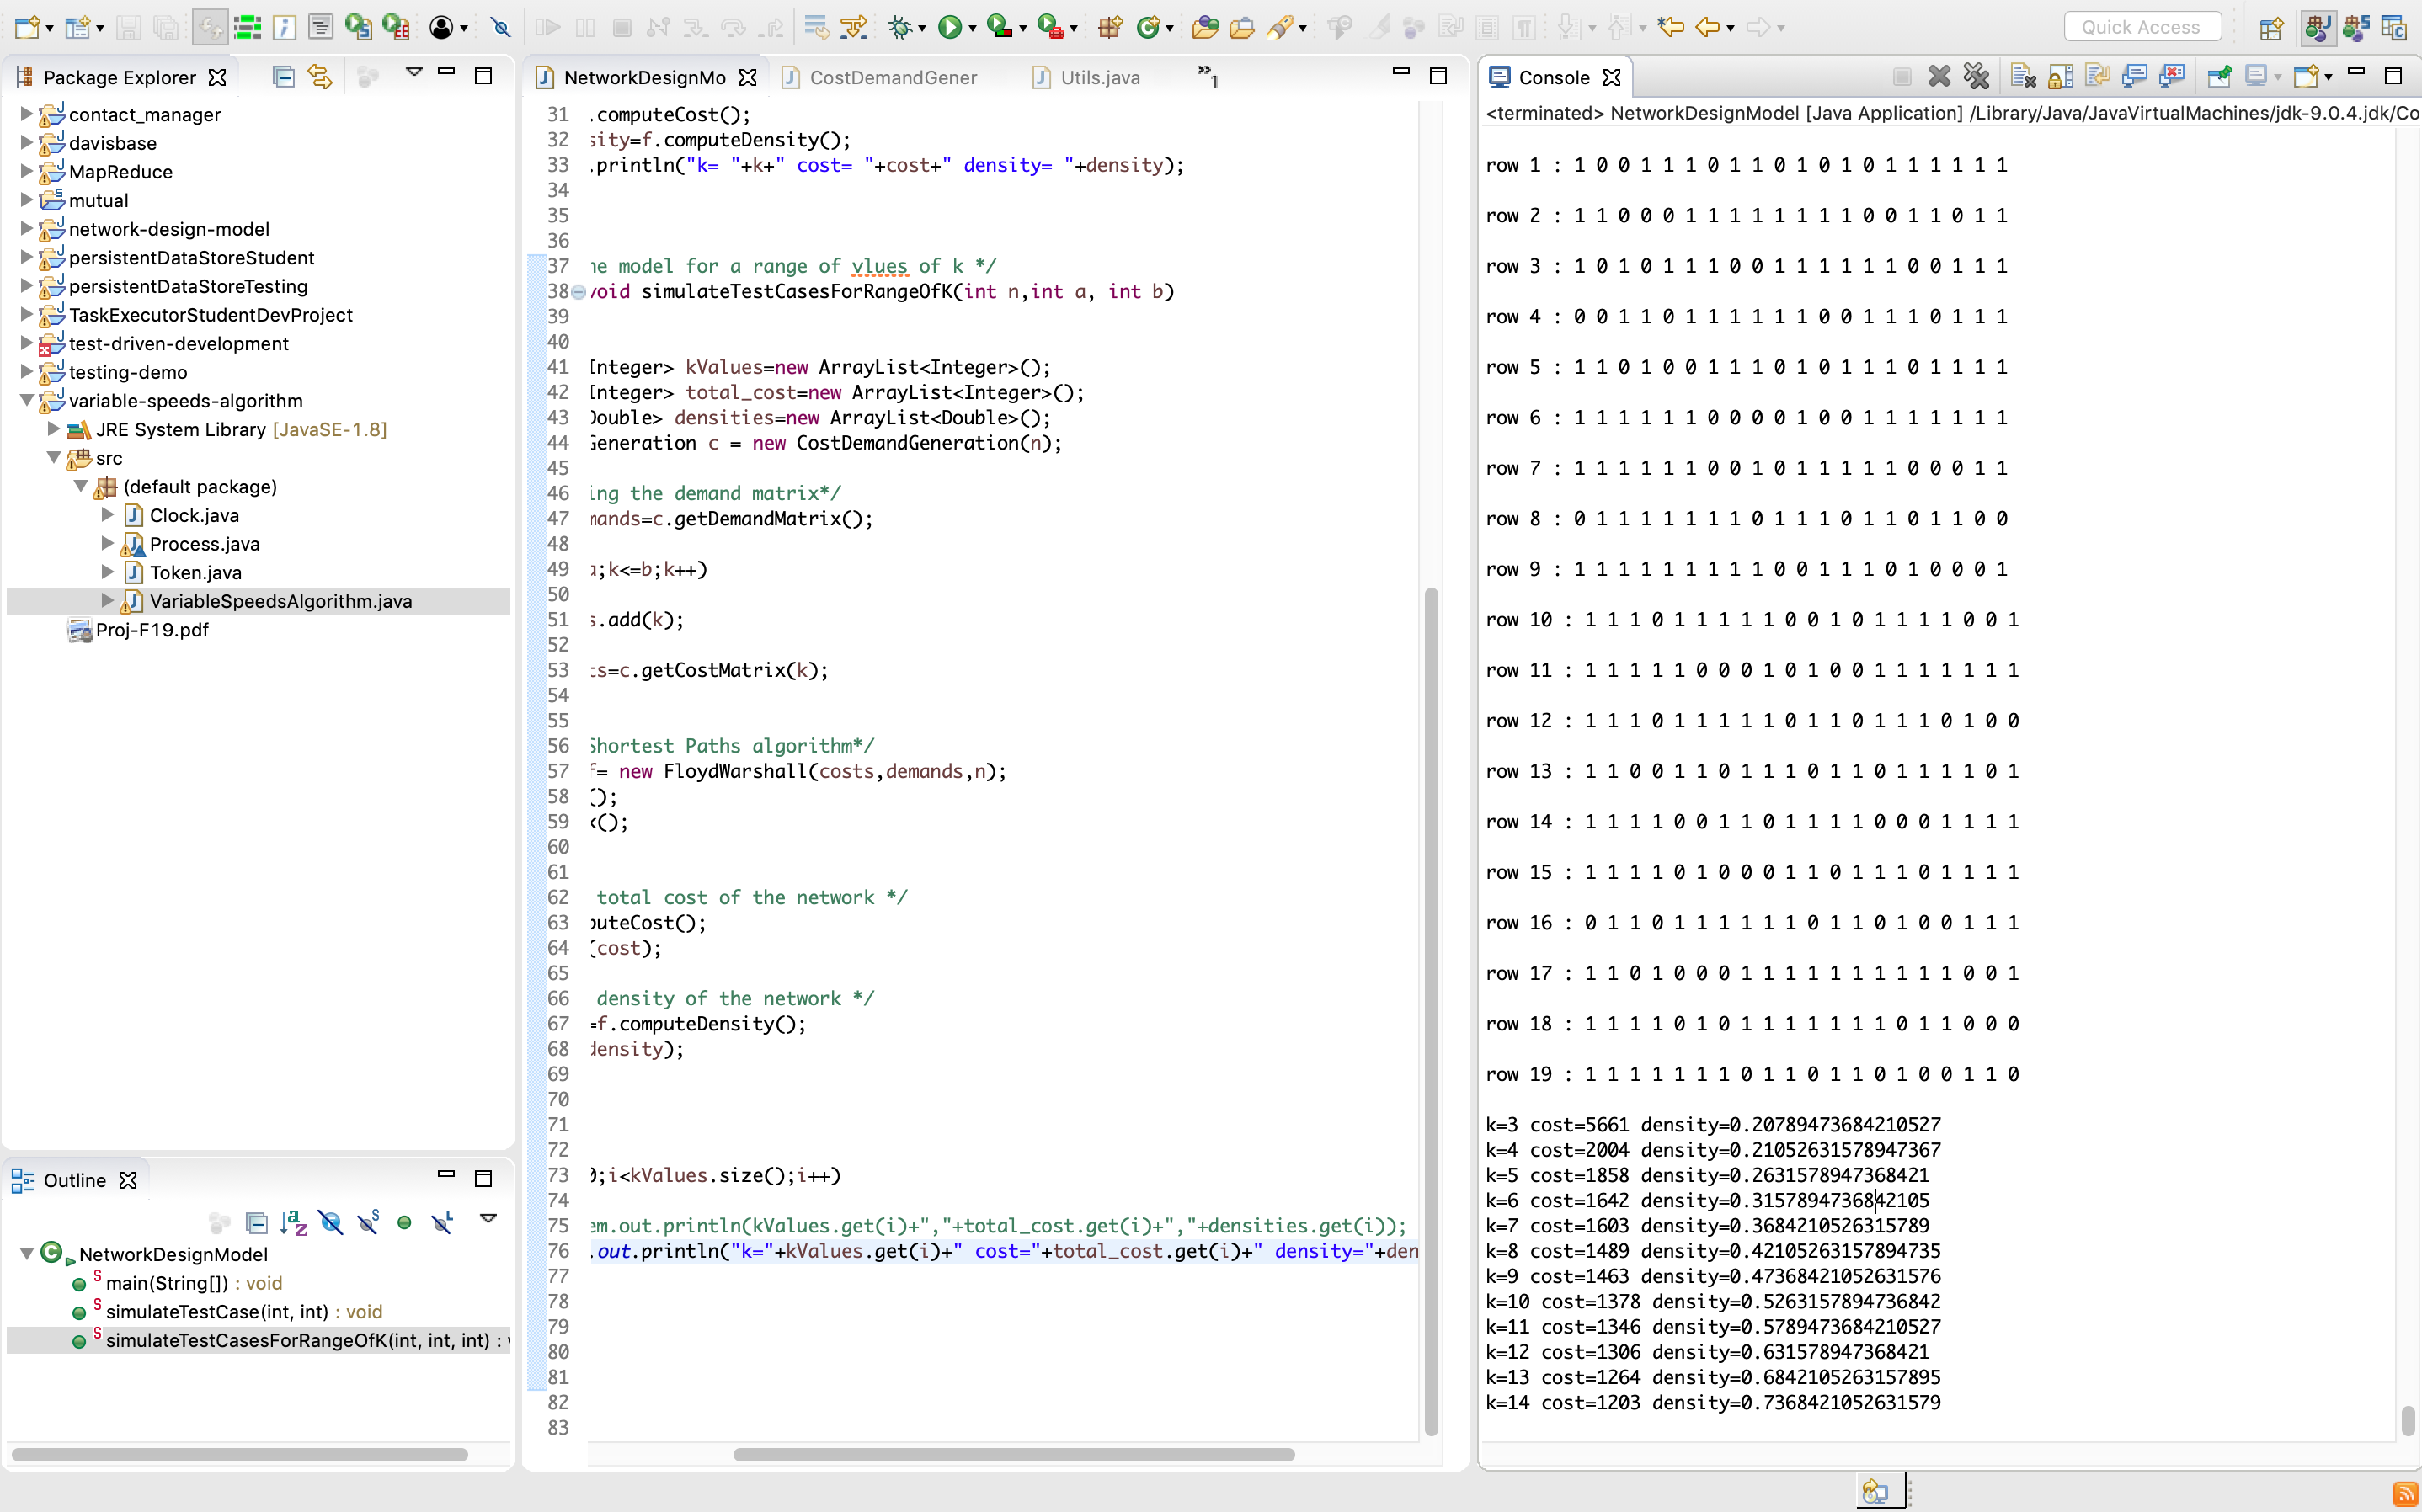
\includegraphics[scale=0.32]{fig/output.png}
 
\item The output results are stored in a \textit{csv} file. The graphs are generated in \textbf{R}.
\item We plot the graph of the parameter \textbf{k} vs. \textbf{cost of the network}. We can clearly see that the cost of the network \textbf{decreases} with increase in the value of k. \\
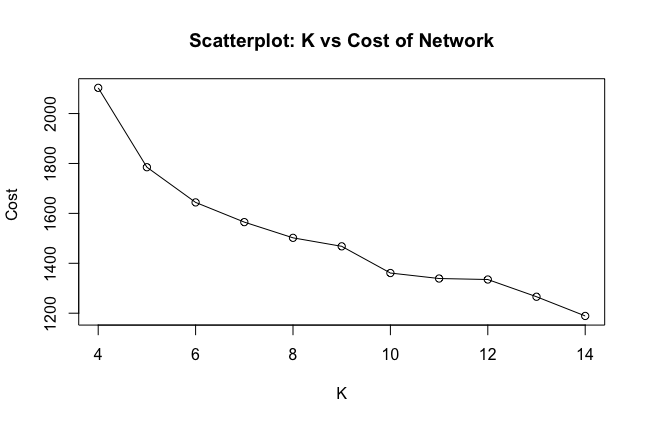
\includegraphics[scale=0.6]{fig/cost.png}

\item We plot the graph of the parameter \textbf{k} against the \textbf{density of the network}. We can clearly see that the density of the network \textbf{increases} with increase in the value of k. \\

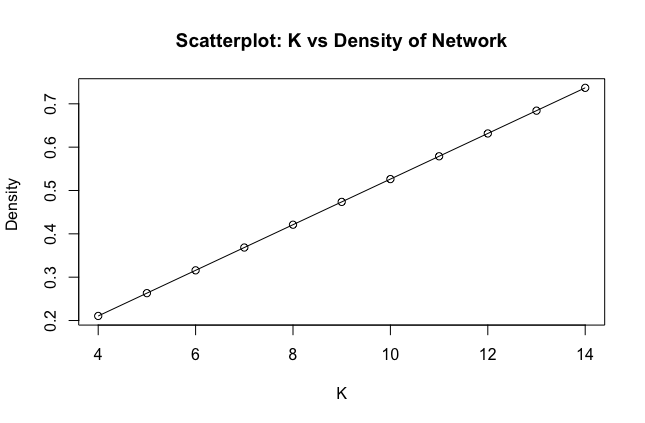
\includegraphics[scale=0.6]{fig/density.png}


\item Network topology for k=3\\

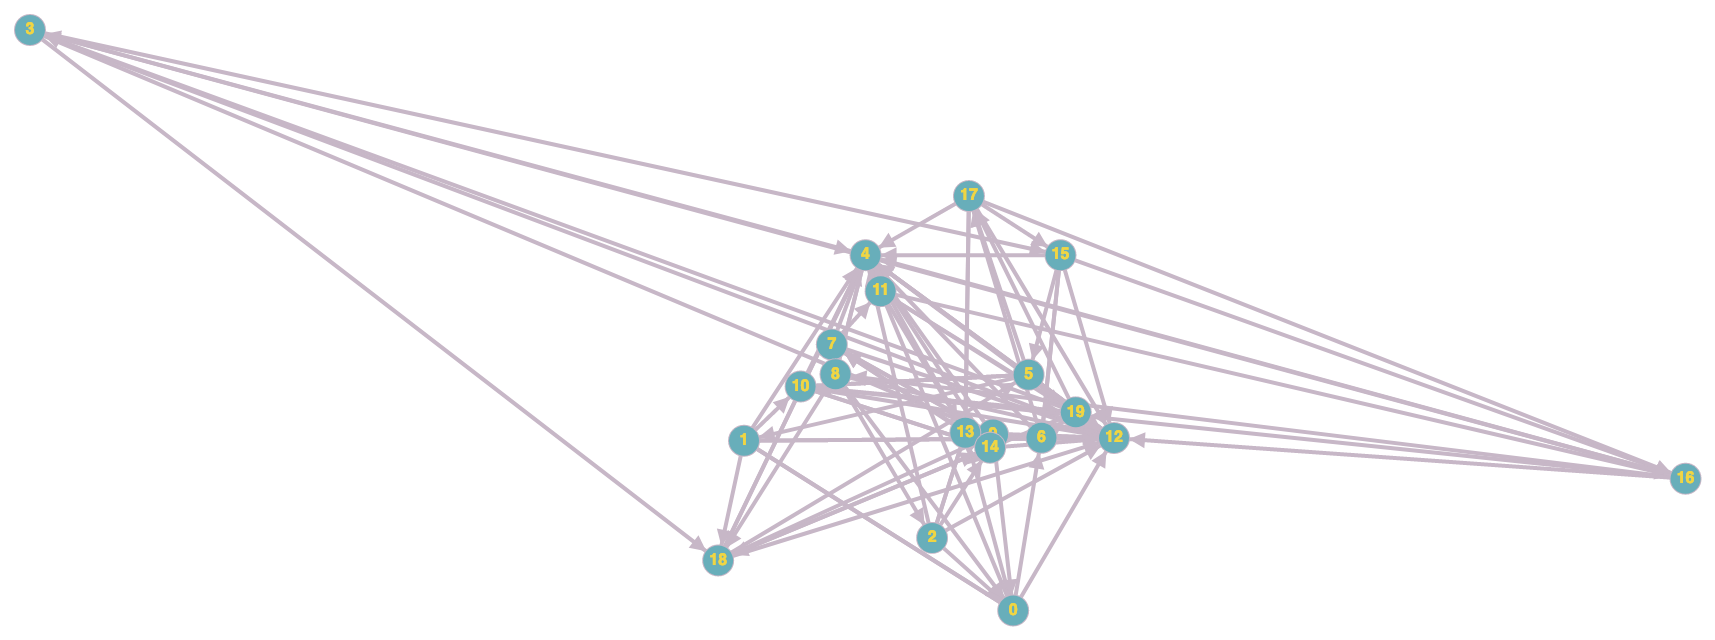
\includegraphics[scale=0.35]{fig/k3.png}

\item Network topology for k=8\\

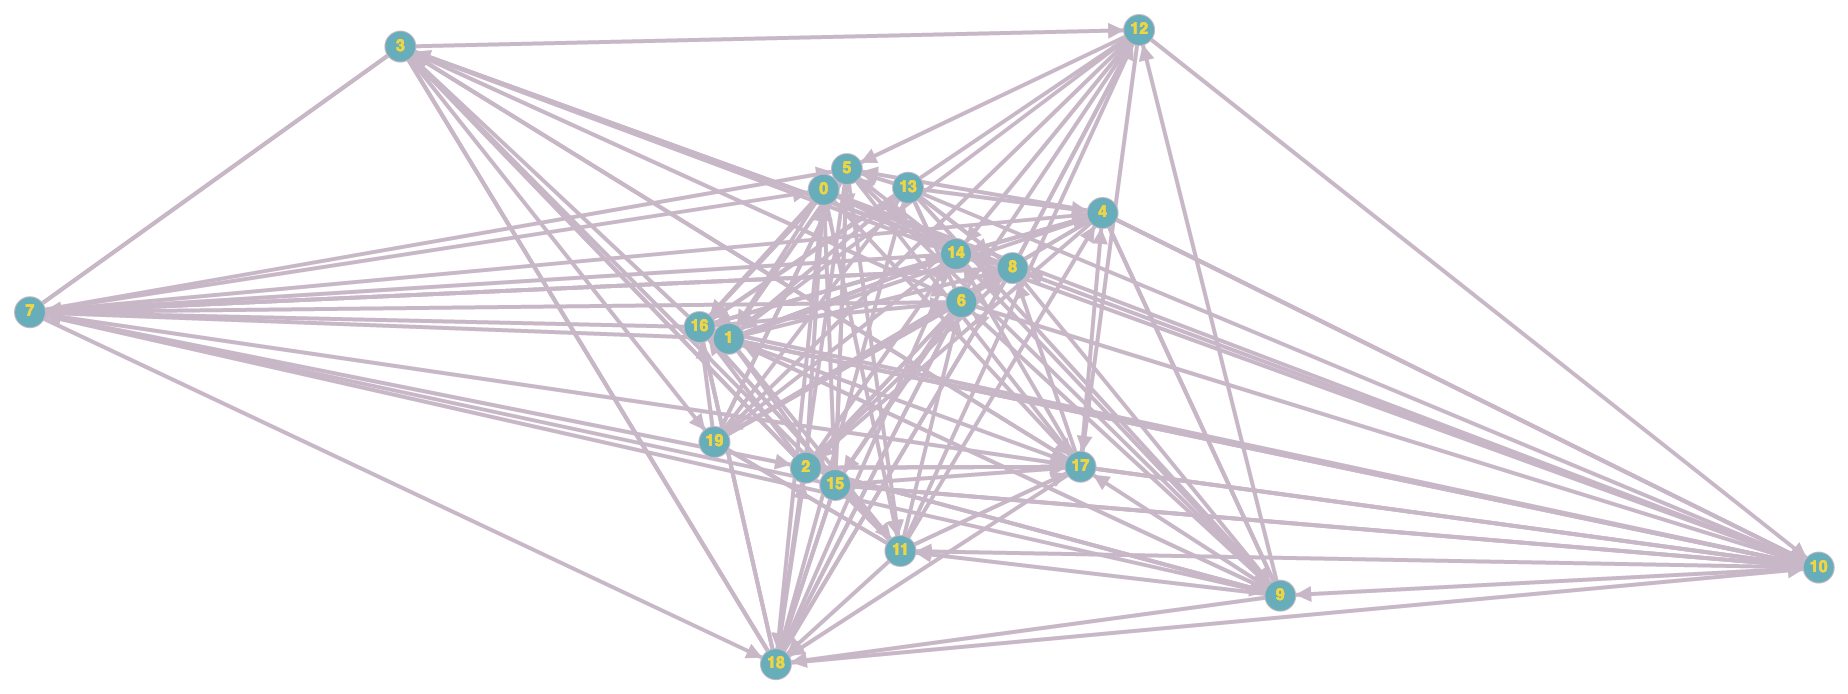
\includegraphics[scale=0.35]{fig/k8.png}


\item Network topology for k=14\\

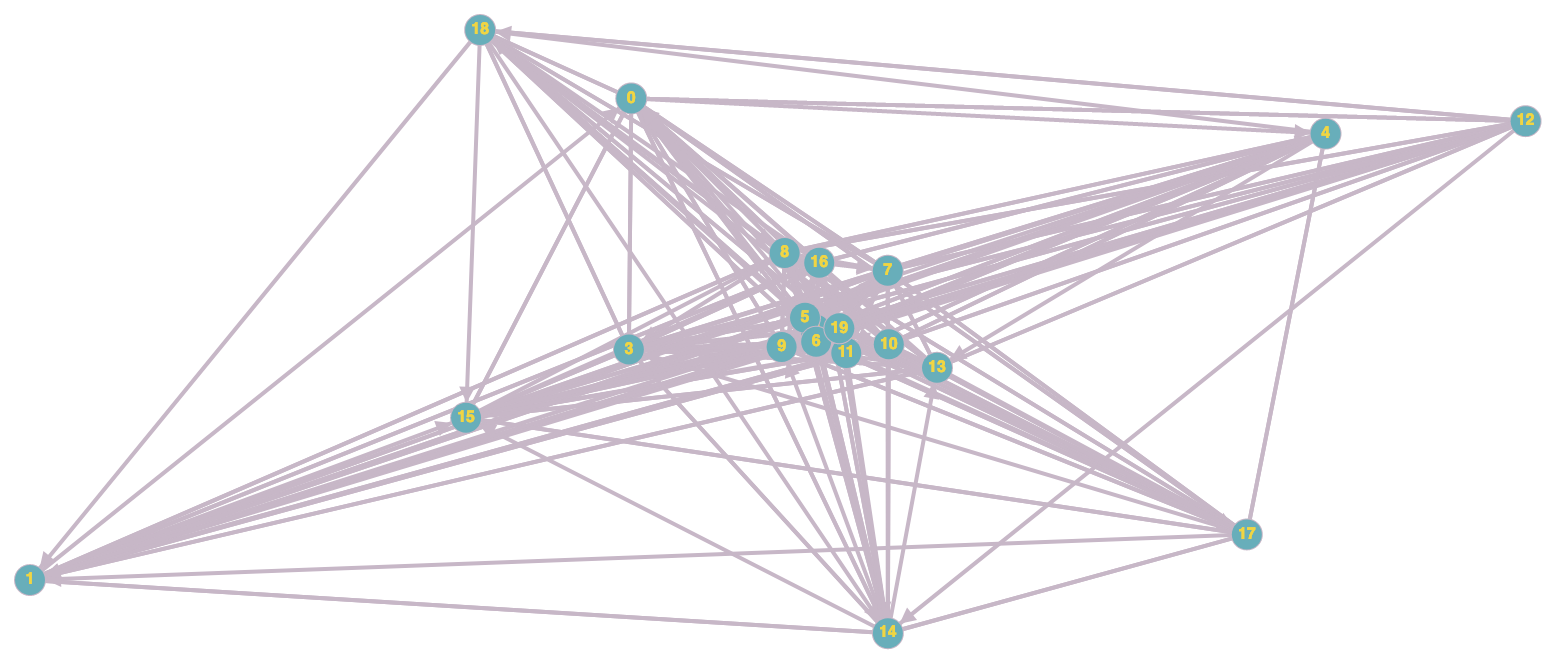
\includegraphics[scale=0.35]{fig/k14.png}

\item We can clearly see that the \textbf{density} of the resulting network \textbf{increases} with increasing value of k.
\end{itemize}
 
\section{Discussion}
\begin{itemize}

\item Consider a single run of our program with any value of k (say k=5). For each node i, there will be 5 low cost links going out of i (cost=1). When the shortest path algorithm executes, it will try to \textbf{avoid} the high cost links (cost=100) going out of node i.

\item Thus by \textbf{limiting k}, we limit the number of links that go out of any node i, and hence limit the \textbf{density} of the network

\item This is the reason we observe that as k \textbf{increases}, the density of our resulting network also \textbf{increases}

\item Consider any pair of nodes (s,t). Let i be any node i on the shortest path from s to t (t cannot be included in this set). As k increases we have more options at all such nodes i to reach t and we could take different paths.

\item The number of edges which repeatedly fall in the shortest path between any 2 pair of nodes \textbf{decreases} and this is why the cost of the network \textbf{decreases}.

\item The network has more of different edges of various edges of different costs rather than few edges some of which may have high costs

\end{itemize}





  \section{ReadMe File}
  This section shows how to run the project files.
  \begin{itemize}
  \item Downloads the project files and store them in a folder
  \item Open the project folder in Eclipse
  \item Open the file \textbf{NetworkDesignModel.java}
  \item Right Click $->$ Run as $->$ Java Application
  \item Alternatively,navigate to the folder in \textbf{terminal} and run the following commands
  \begin{itemize}
  \item javac NetworkDesignModel.java
  \item java NetworkDesignModel
  \end{itemize}
  \end{itemize}

  

 
\section{Code}

\textbf{Module 1: InputGeneration.java}
\lstinputlisting{/users/psprao/eclipse-workspace/Nagamochi-Ibaraki/src/InputGeneration.java}

\pagebreak
\textbf{Module 2: FloydWarshall.java}
\lstinputlisting{/users/psprao/eclipse-workspace/Nagamochi-Ibaraki/src/InputGeneration.java}

\pagebreak
\textbf{Module 3: NetworkDesignModel.java}
\lstinputlisting{/users/psprao/eclipse-workspace/Nagamochi-Ibaraki/src/InputGeneration.java}

\pagebreak
\textbf{Utils.java}
\lstinputlisting{/users/psprao/eclipse-workspace/Nagamochi-Ibaraki/src/Utils.java}

\textbf{Edge.java}
\lstinputlisting{/users/psprao/eclipse-workspace/Nagamochi-Ibaraki/src/Edge.java}


\section{References}
\begin{itemize}


\item Lecture Notes - An Application to Network Design
\end{itemize}


\end{document}
